\newpage

\section{Simulation study}
In this section, HMMs are trained based on the estimation procedure described in \cref{section:estimation}. The primary purpose of the section is to compare how well different estimation methods converge toward the true parameter values, when data is simulated from an HMM. The advantage of using simulated data is that it entails us knowing the true parameter values. Thus, it becomes possible to directly analyze whether a model has learned the estimates close to the true parameter values, as oppossed to relying on general measures of fit, such as AIC and BIC scores, which is necessarily the case when one works with real data. More importantly, simulated data allows us to compare the true state sequences with the estimated. This can be highly informative as it allows the measurement of accuracy in state classification. Simulation will be carried out under various alterations designed to test models' convergence when some of their key assumptions about the data are (partially) unfulfilled\footnote
{Such as the maximum likelihood estimator, which assumes conditional normality. Since it has been shown that e.g. conditional students t-distributions are often a better fit (Bulla, 2011) the assumption is in practice often not fulfilled.
}.

In the following, accuracy of state predictions is defined using recall/sensitivity $\frac{tp}{tp+fn}$, where $tp$ is the number of true positives, and $fn$ is the number of false negative. It measures how large a fraction of all positives that the model is able to detect. When the true state is one, then the positive class will also be one, and the negative class will be all other predictions, when the true state is two the positive class will be two$,\ldots,$ and so on. However, one of the issues with recall is its inability to account for imbalanced data sets. To account for this, Nystrup et al. (2020) suggested using the balanced accuracy score (BAC), which is the average of accuracy in each observed state
\begin{equation}
    BAC = \frac{1}{K} \sum_{k=1}^K \frac{tp_k}{tp_k + fn_k}
\end{equation}
where $tp_k$ is the number of true positives and $fn_k$ is the number of false negatives in state $k$. As a result, when a classifier performs equally well on all states, then BAC reduces to regular accuracy, but if a classifier only performs well by always predicting the dominating class then BAC appropriately drops to the reciprocal of the number of states. So, given data with two classes, then if 99\% of data belongs to the positive class and this is correctly detected, but the remaining 1\% belong to the negative and is incorrectly classified, then that classifier obtains a BAC of 0.50, whereas regular accuracy would be 0.99.

An inherent problem with comparing several HMMs is the fact that, given the unsupervised nature of the model, it outputs label-less states (predictions). This is, not only the case in this simulation study where thousands of models will be compared, but also the case when backtesting e.g. an HMM based on rolling windows on financial data. For example, consider training two HMMs by MLE on the same data with hidden states a and b. Then differences among their final parameter values and state sequences are entirely attributable to the initialized parameter values (as explained in \cref{section:estimation}, which are random quantities. If the models are initialized in a way where the first model labels state a as 1 and state b as 2, whereas the second model might have the order reversed, thus making comparisons of the two (perhaps equally good) models difficult. There are several ways to circumvent this issue, such as choosing the labels that maximize the accuracy score, however since this is impossible to do on real data another method is used here. Since a fundamental assumption in this paper is that the primary difference between conditional gaussian states, is the conditional variance, parameters and state labels are sorted according to variance. Another option could have been sorting according their means, however when thinking about a "good" and "bad" state it is certainly a possibility to observe a state with a high mean and high variance, which we would still interpret as the "bad" state, therefore making such sorting a poor choice.

The rest of the section is structured as follows: First, the simulation procedure is described. Then we describe how to tune the jump penalty $\lambda$ in the jump model. Once the penalty has been tuned, the models can be trained on simulated data and compared. Initially models are trained on correctly specified conditional distributions, after which we show their performance when conditional distributions are purposely misspecified - a feature that is likely when estimating HMMs on real data.

\subsection{Simulation procedure}

Throughout the section, data is simulated from a 2-state HMM. To make results comparable to those of Nystrup et al. (2020), the same parameters are chosen, thus yielding the gaussian HMM
\begin{equation*}
    O_t|S_t \sim N(\mu_{st}, \sigma_{st}^2)
\end{equation*}
with parameters
$$
    \mu_{S_t}=
    \begin{cases}
        \mu_1= 0.0123 \\
        \mu_2= -0.0157
    \end{cases}, \quad
    \sigma_{S_t} =
    \begin{cases}
        \sigma_1 = 0.0347 \\
        \sigma_2 = 0.0778
    \end{cases}, \quad
    \mathbf{A} = 
    \begin{bmatrix}
        0.9629 & 0.0371 \\
        0.2101 & 0.7899
    \end{bmatrix}
$$
The model is estimated by Hardy's (2001) using monthly returns, which has been shown to capture many stylized facts of financial times series such as volatility clustering and leptokurtosis. There is a significant overlap between the two states, making it challenging to correctly infer the unobserved state sequence. By assuming instantaneous log-returns follow a Lêvy process, the parameters are transformed from one time scale $t_1$ to another $t_2$ using
\begin{align*}
    \mu_s(t_1) / t_1 &= \mu_s(t_2) / t_2 \\
    \sigma_s(t_1) / \sqrt{\sigma_s(t_1)} &= \sigma_s(t_2) / \sqrt{\sigma_s(t_2)} \\
    \mathbf{A}(t_1)^{1/t_1} &= \mathbf{A}(t_2)^{1/t_2}
\end{align*}

where $\mu(t), \sigma(t)$ and $\mathbf{A}(t)$ are parameters associated with time scale t. Assuming there is twenty trading days in a month, i.e. $t_{monthly}=20$ and $t_{daily}=1$, monthly parameters are transformed into daily
$$
    \mu_{S_t}=
    \begin{cases}
        \mu_1= 0.0615 \times 10^{-2} \\
        \mu_2= -0.0785 \times 10^{-2}
    \end{cases}, \quad
    \sigma_{S_t} =
    \begin{cases}
        \sigma_1 = 0.7759 \times 10^{-2} \\
        \sigma_2 = 1.7400 \times 10^{-2}
    \end{cases}, \quad
    \mathbf{A} = 
    \begin{bmatrix}
        0.9979 & 0.0021 \\
        0.0120 & 0.9880
    \end{bmatrix}
$$

Each series simulated from this model is generated as follows: The first element $s_0$ is drawn from the stationary distribution $\pi$, and each subsequent element is drawn from $q_{t-1}$, i.e. the row of $Q$ corresponding to the last state sojurn. Based on the value of each $s_t$, observations $o_t$ are generated from the conditional distributions. Concretely, let $\Pi$ denote a realization from the stationary distribution $\pi$. Then

\textbf{Need better notation for the realization from the stationary distribution and from a row of the TPM. http://probcomp.csail.mit.edu/blog/programming-and-probability-sampling-from-a-discrete-distribution-over-an-infinite-set/}

\begin{algorithm}[H]
\KwInput{HMM parameters and sample length H}
 $s_1 = \Pi$ \;
 \For{t=2 to H}{
  $s_t = \alpha_{t-1, j} $\;
   $o_t = N^{-1}(U; \mu_{s_t}, \sigma_{s_t})$ 
 }
\KwOutput{}
\caption{Sampling from an HMM}
\label{algo:sample_hmm}
\end{algorithm}

By repeating this procedure, 1000 different series are simulated with sample lengths $H = 250, 500, 1000, 2000$

\subsection{Choosing the jump penalizer}
\label{subsection: jump_penalizer}

Since the MLE model doesn't have any hyperparameters, it can be applied to the simulated data right away. However, that is not the case for the jump model which requires a given value for $\lambda$. As mentioned previously, we are testing the models' ability to correctly identify state sequences, thus we want to maximize BAC with respect to $\lambda$. Since BAC is a random quantity\footnote
{It is a function of the data and the initial state sequence $s_0$, which in the jump estimator is generated by K-means++. Both quantities are random.
},
we define the estimator $\Omega(\lambda)= \mathbb{E}[BAC|\lambda]$, which is maximized with respect to $\lambda$. This can be estimated by 
\begin{equation}
    \hat\Omega(\lambda) = \frac{1}{N} \sum_{i=1}^N BAC_{i, \lambda}^H
\end{equation}
where N is the amount of simulated series, and $BAC_{i, \lambda}^H$ refer to the BAC of the $i$th sequence of sample size H computed using a jump model with penalty $\lambda$.

We proceed, by computing $BAC_{i, \lambda}^H$ on samples of lengths 250, 500, 1000 and 2000. Further, penalties are considered on a grid defined on the logarithmic scale with base 2. Initially the grid was defined on a logarithmic scale with base 10, but evidently this was too course to yield meaningful results. Grid points are equidistantly placed on the closed interval $[2^{-2}, 2^{7}]$. Results are shown in \cref{fig:jump_penalties}. As evident by the figure, the primary difference between simulation lengths is the size of BAC, which is generally increasing with sample size. Once $\lambda$ is below a certain threshold, in this case around $2^5$, BAC isn't too sensitive to the precise level of the penalty. As noted earlier, when $\lambda$ is sufficiently small, BAC converges to the unpenalized case, which is essentially the same as applying a K-means model where the time ordering of observations is irrelevant. For $\lambda$ too large, the jump estimator only identifies the dominating state, and as a result BAC drops to 0.50. 

\begin{figure}[H]
    \centering
    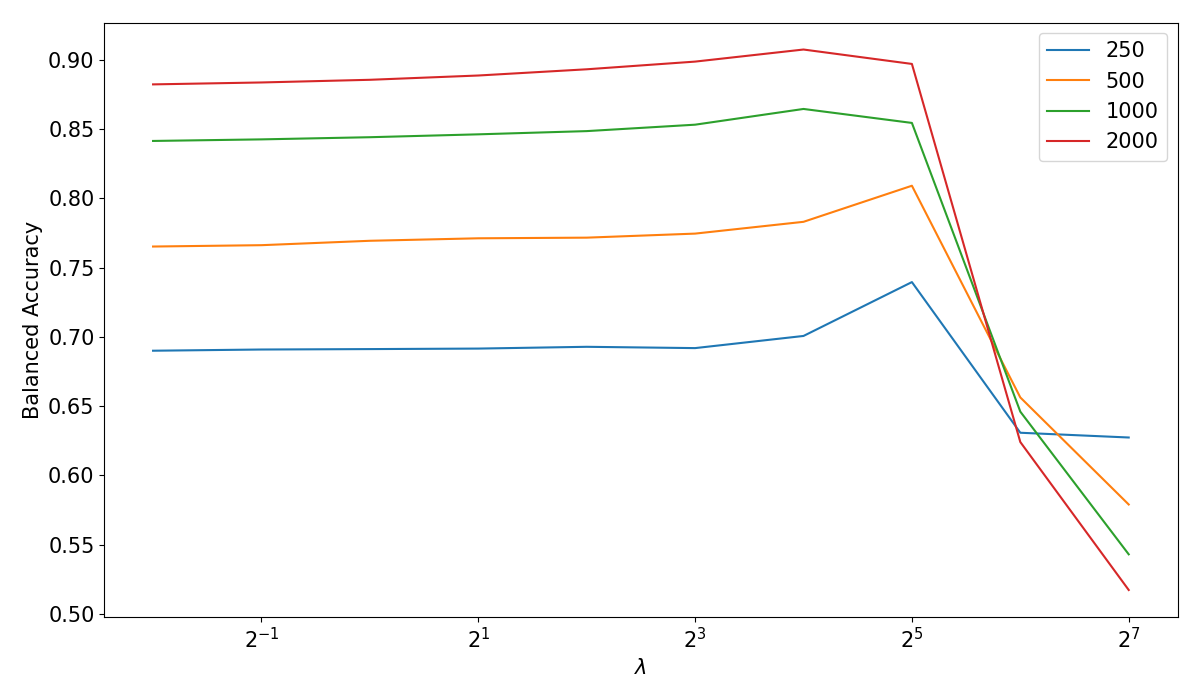
\includegraphics[width=1\textwidth]{analysis/model_convergence/images/jump_penalties.png}
    \caption{Balanced accuracy of jump estimator, as a function of the penalty $\lambda$ using different simulation lengths. All points are based on the estimate $\hat\Omega(\lambda)$ based on 1000 simulated series.}
    \label{fig:jump_penalties}
\end{figure}

From \cref{fig:jump_penalties}, the optimal level of $\lambda$ is roughly equivalent for all simulation lengths, though for $H=250,500$, the optimal penalty is bit higher. As the difference is still quite small, and more importantly, due to the large drop in BAC across all simulation lengths for $\lambda > 2^5$, the optimal penalty is chosen as $\lambda=2^4$ for all simulation lengths. 

\textbf{Consider discussing time-variation in $\lambda$ and how the size of $\lambda$ relates to the size of means in feature matrix.}

\subsection{Simulation study with correctly specified distributions}

\cref{tab:jump_gaussian} summarizes the performance of the MLE and Jump estimator for various sample sizes when compared to the true values. Apart from the HMM parameters, the accuracy in each state as well as BAC is reported. Accuracy for for the true parameters are obtained by running the Viterbi algorithm using an HMM with the true model parameters. This can be seen as the best obtainable performance in state detection and is used to get a sense of where the 'upper bound' on BAC lies when comparing the other models.

\begin{table}[H]
\centering
\caption{Estimated model parameters based on 1000 different simulations from conditional gaussian distributions}
\begin{tabular}{llrrrrrr}
\toprule
     &      &  $\mu_1$ &  $\mu_2$ &  $\sigma_1$ &  $\sigma_2$ &  $q_{11}$ &  $q_{22}$ \\
sample_size & model &          &          &             &             &           &           \\
\midrule
250  & true &   0.0006 &  -0.0008 &      0.0078 &      0.0174 &    0.9979 &    0.9880 \\
     & mle &   0.0017 &  -0.0000 &      0.0052 &      0.0121 &    0.7410 &    0.9658 \\
     & jump &   0.0006 &  -0.0001 &      0.0079 &      0.0113 &    0.9770 &    0.8903 \\
500  & true &   0.0006 &  -0.0008 &      0.0078 &      0.0174 &    0.9979 &    0.9880 \\
     & mle &   0.0015 &  -0.0002 &      0.0060 &      0.0139 &    0.8152 &    0.9719 \\
     & jump &   0.0006 &  -0.0003 &      0.0079 &      0.0130 &    0.9834 &    0.8898 \\
1000 & true &   0.0006 &  -0.0008 &      0.0078 &      0.0174 &    0.9979 &    0.9880 \\
     & mle &   0.0011 &  -0.0006 &      0.0071 &      0.0160 &    0.9208 &    0.9763 \\
     & jump &   0.0006 &  -0.0006 &      0.0080 &      0.0152 &    0.9866 &    0.9420 \\
2000 & true &   0.0006 &  -0.0008 &      0.0078 &      0.0174 &    0.9979 &    0.9880 \\
     & mle &   0.0008 &  -0.0007 &      0.0076 &      0.0171 &    0.9823 &    0.9817 \\
     & jump &   0.0006 &  -0.0007 &      0.0080 &      0.0164 &    0.9951 &    0.9679 \\
\bottomrule
\end{tabular}

\label{tab:jump_gaussian}
\end{table}

\begin{figure}[H] 
    \centering
    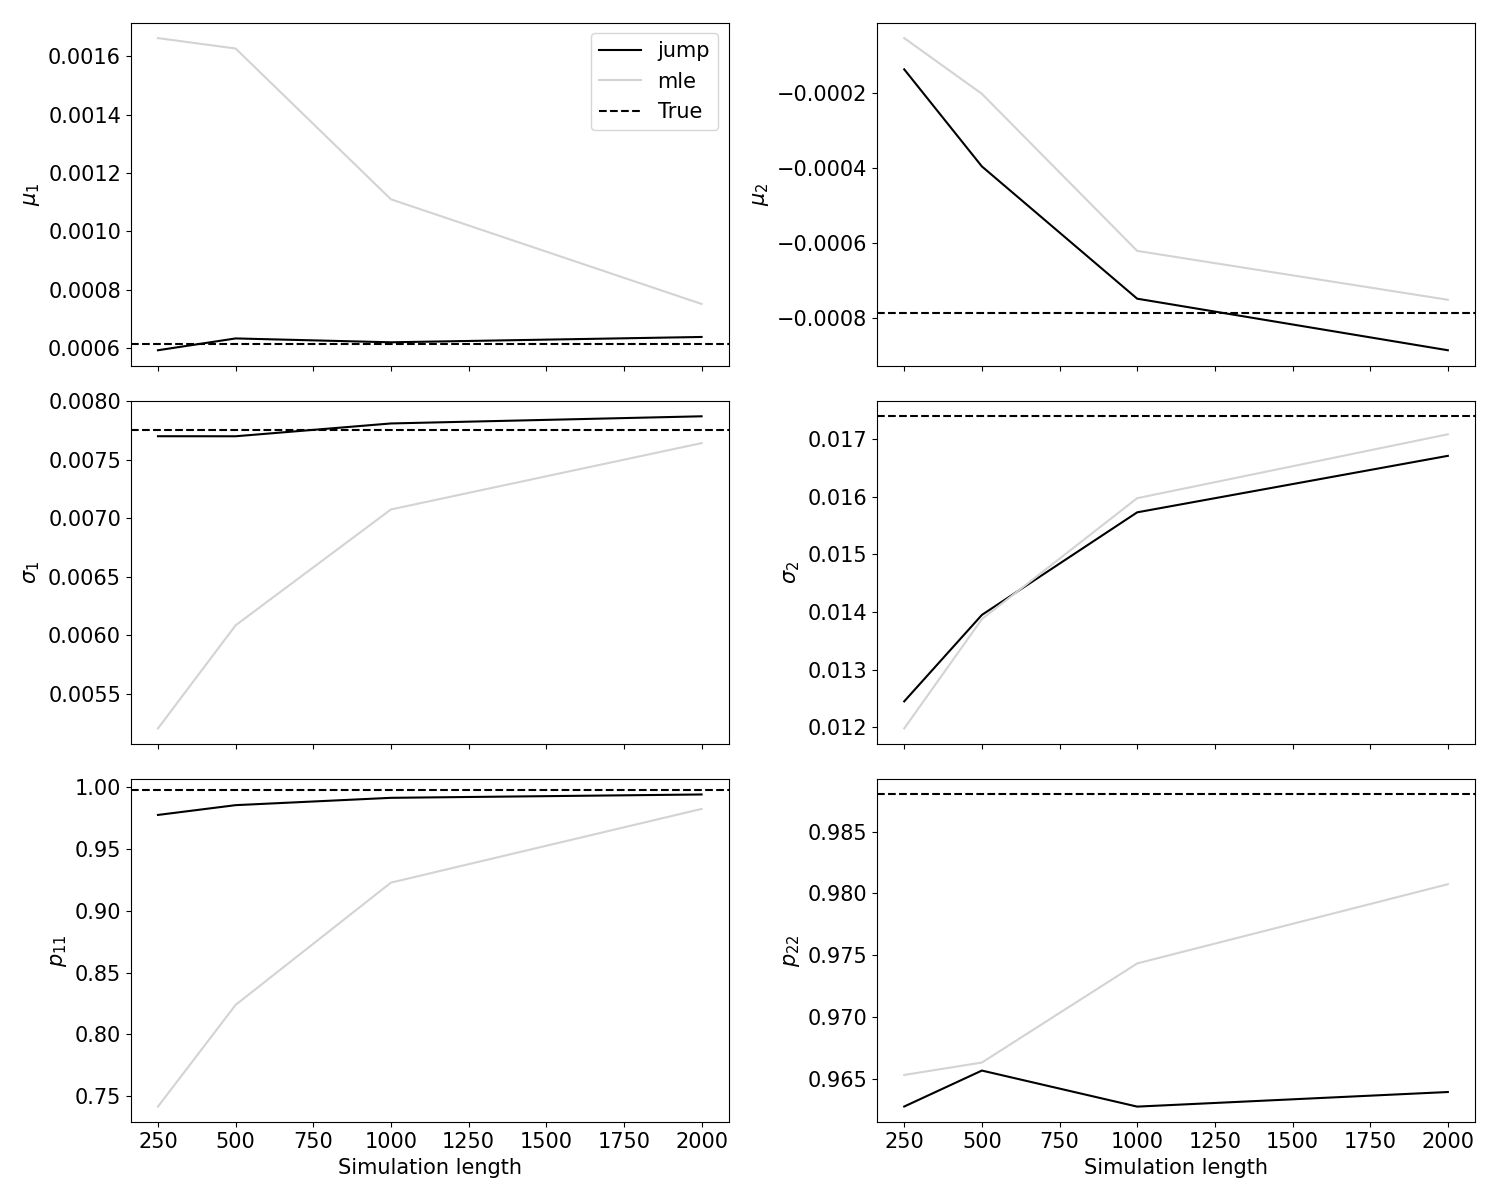
\includegraphics[width=1\textwidth]{analysis/model_convergence/images/simulation_normal.png}
    \caption{Hyper-tuning.}
    %\label{fig:jump_penalties}
\end{figure}



\subsection{Simulation study with misspecified distributions}

\begin{figure}[H] 
    \centering
    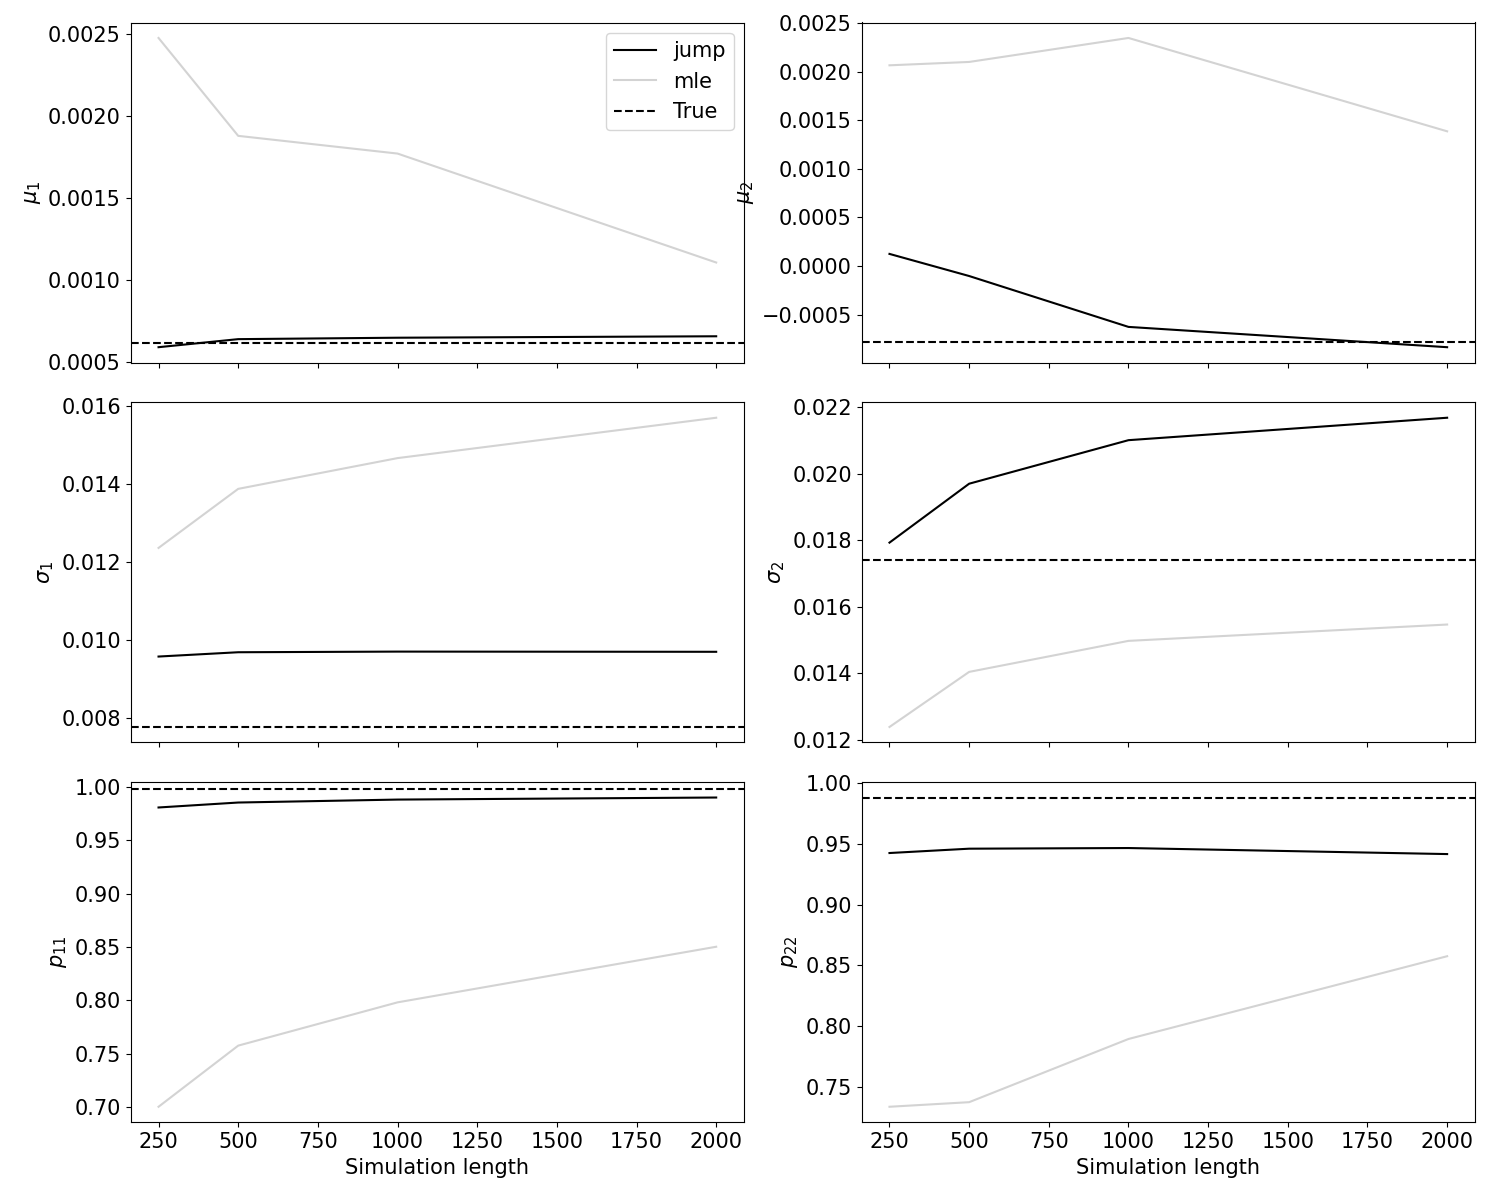
\includegraphics[width=1\textwidth]{analysis/model_convergence/images/simulation_t.png}
    \caption{Estimated mean model parameters based on 1000 different simulations from conditional t-distributions with five degrees of freedom}
    %\label{fig:jump_penalties}
\end{figure}

\begin{table}[H]
\centering
\caption{Estimated mean model parameters based on 1000 different simulations from conditional t-distributions}
\begin{tabular}{llrrrrrr}
\toprule
     &      &   $\mu_1$ &   $\mu_2$ &  $\sigma_1$ &  $\sigma_2$ &    $q_11$ &    $q_22$ \\
sample_size & model &           &           &             &             &           &           \\
\midrule
250  & true &  0.000615 & -0.000785 &    0.007759 &    0.017397 &  0.997900 &  0.988000 \\
     & mle &  0.002475 &  0.002068 &    0.012354 &    0.012383 &  0.700296 &  0.733797 \\
     & jump &  0.000591 &  0.000125 &    0.009567 &    0.017927 &  0.980719 &  0.942377 \\
500  & true &  0.000615 & -0.000785 &    0.007759 &    0.017397 &  0.997900 &  0.988000 \\
     & mle &  0.001878 &  0.002102 &    0.013870 &    0.014039 &  0.757573 &  0.737563 \\
     & jump &  0.000640 & -0.000103 &    0.009677 &    0.019699 &  0.985360 &  0.945942 \\
1000 & true &  0.000615 & -0.000785 &    0.007759 &    0.017397 &  0.997900 &  0.988000 \\
     & mle &  0.001769 &  0.002351 &    0.014671 &    0.014961 &  0.797976 &  0.789653 \\
     & jump &  0.000648 & -0.000627 &    0.009694 &    0.021009 &  0.988130 &  0.946477 \\
2000 & true &  0.000615 & -0.000785 &    0.007759 &    0.017397 &  0.997900 &  0.988000 \\
     & mle &  0.001107 &  0.001388 &    0.015695 &    0.015464 &  0.850219 &  0.857551 \\
     & jump &  0.000657 & -0.000836 &    0.009689 &    0.021683 &  0.990051 &  0.941516 \\
\bottomrule
\end{tabular}

\end{table}